\documentclass{report}

\title{Mécatro: Rapport d'automatique}
\author{Groupe 7: Royer Jules, Simon Noah-Luc, Colin Matthieu, Bourderioux Armand}

\date{}

\usepackage[T1]{fontenc}
\usepackage{lmodern}

\usepackage[margin=0.7in]{geometry}

\usepackage{amssymb}
\usepackage{gensymb}
\usepackage{mathrsfs}

\usepackage{amsmath}
\usepackage{mathtools}

\usepackage{graphicx}
\usepackage{float}

\usepackage[parfill]{parskip}

\preto{\subsection}{\Needspace{5\baselineskip}}
\preto{\section}{\Needspace{5\baselineskip}}

\hyphenpenalty=10000

\usepackage{listings}
\usepackage{pxfonts}

\usepackage{biblatex}
\addbibresource{bibliography.bib}

\usepackage{blindtext}

\usepackage{hyperref}

\begin{document}

\maketitle

\tableofcontents

\chapter{Introduction}
Le but de la partie automatique du projet de mécatronique est de créer un contrôleur
pour un robot "bolide" suiveur de ligne. Le contrôleur a d'abord été créé théoriquement
dans le logiciel Matlab et testé sur un modèle de simulation Simulink, puis il a été
implémenté informatiquement en Arduino afin d'être embarqué dans le robot.

\chapter{Création du contrôleur théorique}

\paragraph{Contrôle d'un mouvement rectiligne uniforme}

En reprenant les notations et la modélisation du document "Equations de la dynamique du Segway",
les équations de la dynamique sous forme d'état sont:

\begin{equation*}
    \begin{cases}
        \dot{p} = u \\
        \dot{u} = \frac{1}{\beta}\big( \frac{1}{\rho}kI^{+} - m_bdv^2 \big) \\
        \dot{\psi} = v \\
        \dot{v} = \frac{1}{\gamma}\big( \frac{lk}{2\rho}I^{-} + m_bduv \big) \\
        \dot{I^{+}} = \frac{U^{+}}{L} - \frac{R}{L}I^{+} - \frac{2k}{L\rho}u \\
        \dot{I^{-}} = \frac{U^{-}}{L} - \frac{R}{L}I^{-} - \frac{kl}{L\rho}v \\
        \dot{y} = u\sin\psi \\
    \end{cases}
\end{equation*}

Les entrées sont $U^{+}$, $U^{-}$.

Les sorties mesurées sont:

\begin{equation*}
    \begin{cases}
        \delta \delta \phi^{+} = \delta \phi_{right} + \delta \phi_{left} = \frac{2}{\rho}p \\
        \delta \delta \phi^{-} = \delta \phi_{right} + \delta \phi_{left} = \frac{l}{\rho}\psi \\
        c_{LF} = \frac{y}{\cos\psi} \approx y \\
    \end{cases}
\end{equation*}

Où on a défini:

\begin{itemize}
    \item $p$ la distance curviligne parcourue par le robot le long de sa trajectoire.
    Celle-ci doit figurer dans l'état pour mesurer les angles cumulés.
    \item $u$ sa vitesse longitudinale.
    \item $\psi$ l'angle entre l'axe horizontal $x$ et la direction du robot.
    \item $I^{-} = I_{right} - I_{left}$ la somme des courants des moteurs.
    \item $I^{-} = I_{right} - I_{left}$ la différence des courants.
    \item $U^{+} = U_{right} + U_{left}$ la somme des tensions aux bornes des moteurs.
    \item $U^{-} = U_{right} - U_{left}$ la différence des tensions.
    \item $\beta = M + \frac{2I^{w}_{y}}{\rho^2}$
    \item $\gamma = I_{\psi} + m_bd^2$
    \item $\delta \delta \phi^{+}$ la somme des angles des roues. Posons $\alpha = \frac{2}{\rho}$.
    \item $\delta \delta \phi^{-}$ la différence des angles des roues. Posons  $\eta = \frac{l}{\rho}$.
    \item $c_{LF}$ la mesure de l'écart entre le point A et la ligne (approximation en MRU horizontal).
\end{itemize}


\begin{figure}[h]  % Placement "here"
    \centering
    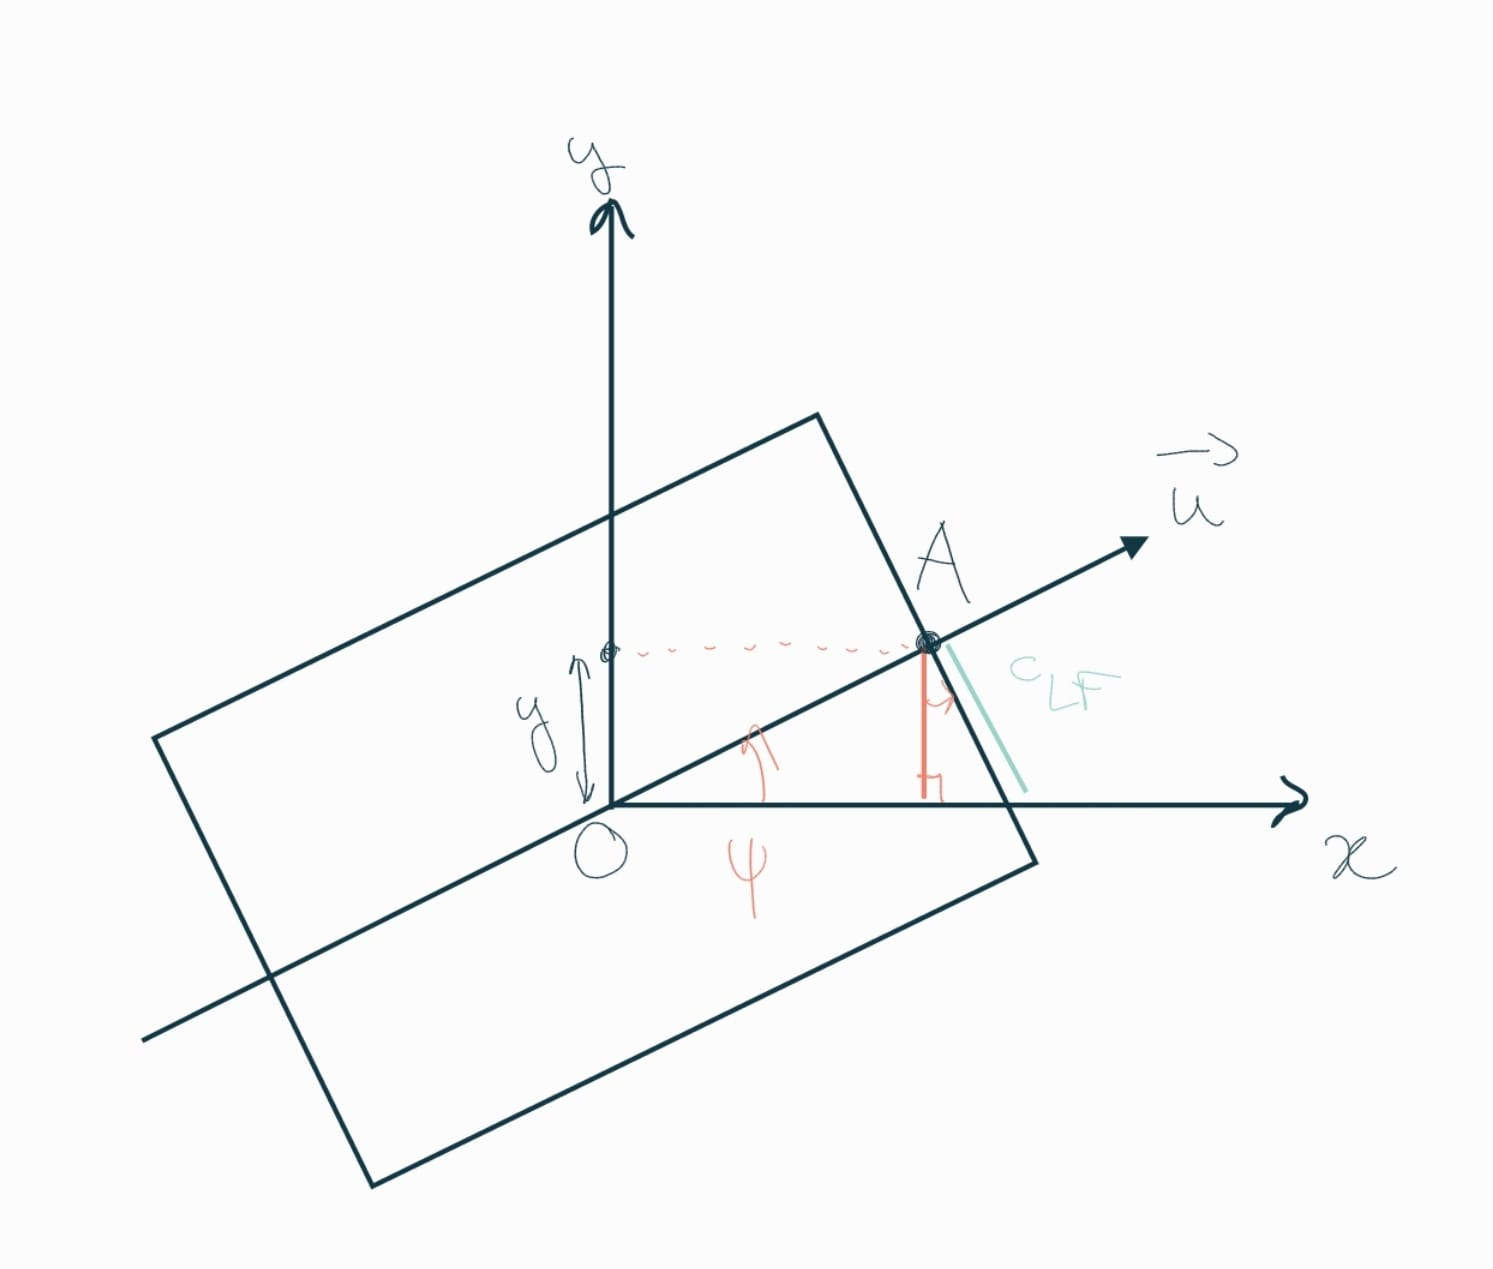
\includegraphics[width=0.5\textwidth]{figures/cLF_schema.jpg}
    \caption{Ecart à la ligne dans l'hypothèse d'un faible angle.}
\end{figure}


\paragraph{Recherche des trajectoires d'équilibre}

Notre trajectoire d'équilibre du mouvement rectiligne uniforme 
est caractérisée par le système:

\begin{equation*}
    \begin{cases}
        u_0 = \overline{u} \\
        0 = \frac{1}{\beta}\big( \frac{1}{\rho}k\overline{I^{+}} - m_bd\overline{v}^2 \big) \\
        0 = \overline{v} \\
        0 = \frac{1}{\gamma}\big( \frac{lk}{2\rho}I^{-} + m_bd\overline{u}\overline{v} \big) \\
        0 = \frac{\overline{U^{+}}}{L} - \frac{R}{L}\overline{I^{+}} - \frac{2k}{L\rho}\overline{u} \\
        0 = \frac{\overline{U^{-}}}{L} - \frac{R}{L}\overline{I^{-}} - \frac{kl}{L\rho}\overline{v} \\
        0 = \overline{u}\sin\overline{\psi} \\
    \end{cases}
\end{equation*}

Avec les sorties linéarisées:

\begin{equation*}
    \begin{cases}
        \delta \phi^{+} = \alpha \delta p \\
        \delta \phi^{-} = \eta \delta \psi \\
        \delta c_{LF} = \delta y \\
    \end{cases}
\end{equation*}

Ce qui donne comme trajectoire d'équilibre 
\begin{equation*}
    \begin{cases}
        \underline{x} = \big(\overline{p}=u_0t, \overline{u}=0, \overline{\psi}=\psi_0=0, 
        \overline{v}=0, \overline{I^{\pm}}=0, \overline{y}=0 \big) \\
        \underline{e} = \big( \overline{U^{+}}=\frac{2k}{\rho} u_0, \overline{U^{-}}=0 \big)
    \end{cases}
\end{equation*}

\paragraph{Linéarisé autour de l'équilibre}

\begin{equation*}
    \begin{cases}
        \delta{\dot p} = \delta u \\
        \delta{\dot u} = \frac{1}{\beta}\frac{1}{\rho}k\delta I^{+} \\
        \delta{\dot \psi} = \delta v \\
        \delta{\dot v} = \frac{1}{\gamma}\big( \frac{lk}{2\rho}\delta I^{-} + m_bd u_0 \delta v \big) \\
        \delta{\dot I^{+}} = \frac{\delta U^{+}}{L} - \frac{R}{L}\delta I^{+} - \frac{2k}{L\rho}\delta u \\
        \delta{\dot I^{-}} = \frac{\delta U^{-}}{L} - \frac{R}{L}\delta I^{-} - \frac{kl}{L\rho}\delta v \\
        \dot{y} = u_0\cos\psi_0 \delta \psi + \delta u \sin\psi_0 = u_0 \delta \psi \\
    \end{cases}
\end{equation*}

\paragraph{Simplifications par perturbations singulières}

Les intensités de courant ont un transitoire bien plus rapide que
ceux des grandeurs mécaniques (leurs valeurs propres $\frac{R}{L}$ sont bien supérieures aux autres).

\begin{figure}[h]  % Placement "here"
    \centering
    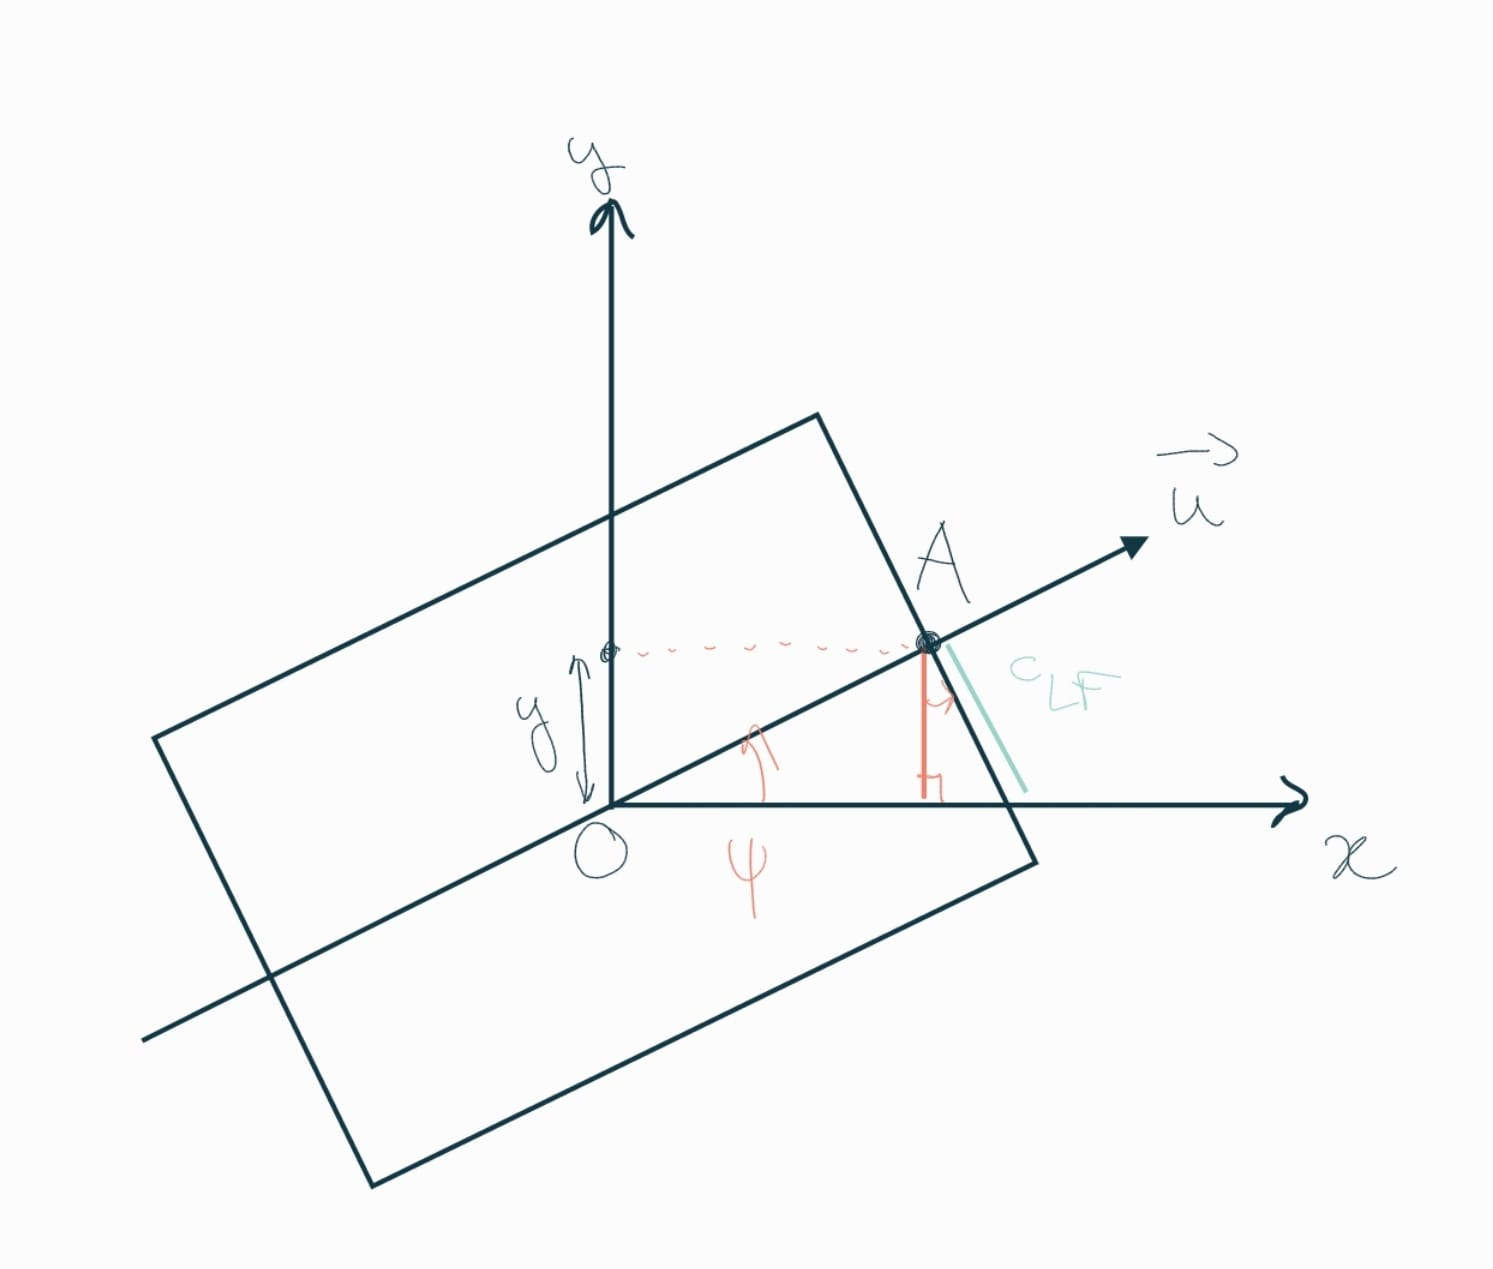
\includegraphics[width=0.5\textwidth]{figures/cLF_schema.jpg}
    \caption{Valeurs propres du système modélisé dans Matlab}
\end{figure}

On applique la méthode des perturbations singulières à:
\begin{equation*}
    \begin{cases}
        L\dot{I^{+}} = U^{+} - RI^{+} - \frac{2k}{\rho}u \\
        L\dot{I^{-}} = U^{-} - RI^{-} - \frac{kl}{\rho}v \\
    \end{cases}
\end{equation*}

Avec $\varepsilon = L$ "très petit". En tout rigueur il faudrait introduire
$L_0$ pour adimensionner $\varepsilon$.

On obtient:

\begin{equation*}
    \begin{cases}
        I^{+} = \frac{1}{R} \big(U^{+} - \frac{2k}{\rho}u \big) \\
        I^{-} = \frac{1}{R} \big(U^{-} - \frac{kl}{\rho}v \big)\\
    \end{cases}
\end{equation*}

On vérifie la stabilité uniformément exponentielle de la branche d'équilibre avec :

\begin{equation*}
    \partial_{I^{\pm}}
    \begin{pmatrix}
        \frac{U^{+}}{L} - \frac{R}{L}I^{+} - \frac{2k}{L\rho}u  \\
        \frac{U^{-}}{L} - \frac{R}{L}I^{-} - \frac{kl}{L\rho}v  
    \end{pmatrix} \biggr\rvert_{I^{\pm} = f(\underline{x}, \underline{e})}
    = -\frac{R}{L}
    \begin{pmatrix}
        1 & 0 \\
        1 & 0
    \end{pmatrix}
\end{equation*}

La branche a donc comme valeurs propres des réels négatifs, donc est ue-stable.

\paragraph{Système lent simplifié}

\begin{equation*}
    \begin{cases}
        \dot{p} = u \\
        \dot{u} = \frac{1}{\beta}\big( \frac{1}{\rho}kI^{+} - m_bdv^2 \big) \\
        \dot{\psi} = v \\
        \dot{v} = \frac{1}{\gamma}\big( \frac{lk}{2\rho}I^{-} + m_bduv \big) \\
        \dot{I^{+}} = \frac{U^{+}}{L} - \frac{R}{L}I^{+} - \frac{2k}{L\rho}u \\
        \dot{I^{-}} = \frac{U^{-}}{L} - \frac{R}{L}I^{-} - \frac{kl}{L\rho}v \\
        \dot{y} = u\sin\psi \\
    \end{cases}
\end{equation*}



\chapter{Identification des paramètres physiques}

Nous avons rassemblé toutes les valeurs numériques dans ce 
\href{https://docs.google.com/spreadsheets/d/1PVCPAeFXgacQK3YaMxcYYtDlWB_0VT0cpRnJDznpAQc/edit?pli=1#gid=0
}{Google Sheet}.

\paragraph{Estimation de la constante de couple k}

Les équations électriques à l'équilibre s'écrivent

\begin{equation*}
    \begin{cases}
        0 = U - RI - k\Omega \\
        \tau = kI       
    \end{cases}
\end{equation*}

En se plaçant sans couple, donc sans courant, et en utilisant les courbes constructeurs, on calcule
$k=\frac{U}{\Omega} \, V/(rad.s^-1)$.

\begin{figure}[h]  % Placement "here"
    \centering
    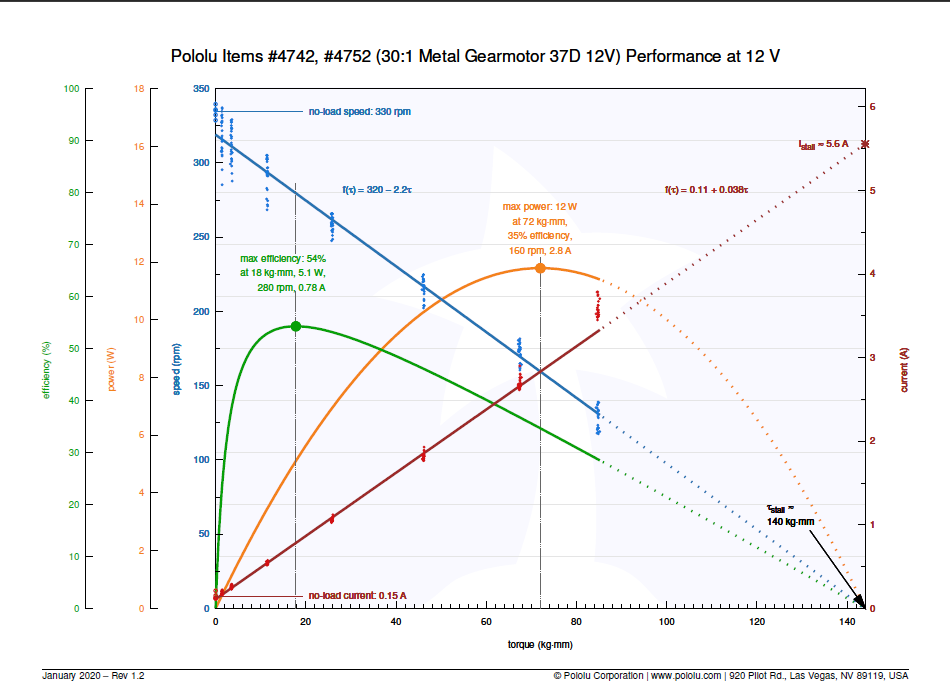
\includegraphics[width=3cm]{figures/courbes-construc.png}
    \caption{Courbes de fonctionnement fournies par Pololu.}
\end{figure}

\paragraph{Estimation des masses des pièces}
Toutes les pièces ont été pesées.

On a approximé la masse de l'arbre moteur et du rotor à la différence
entre la masse pesée du moteur, et celle donnée par la CAO.

\paragraph{Estimation des moments d'inertie}

Pour le moment d'inertie de l'unité roue + engrenage + rotor, 
notre première approche a été d'approximer la géométrie du système à celle d'un disque,
et d'utiliser la matrice d'inertie (cellule D34 du GSheet):

\begin{equation*}
    I_w(C_w) = 
    \begin{pmatrix}
        m \big(\rho^2/4 + l_w^2/2 \big) & 0 & 0 \\
        0 & m \big(\rho^2/4 + l_w^2/2 \big) & 0 \\
        0 & 0 & m \big(R^2/4 + l^2/12 \big)
    \end{pmatrix}
\end{equation*}

Comme autre approche, nous avons mesuré le temps de réponse de la 
vitesse angulaire de la roue à un échelon de 12V aux bornes du moteur.
Nous avons mesuré la sommes des positions angulaires, que nous avons filtrée 
avec un filtre passe bas, en supposant que cela ne fausse pas sensiblement le 
temps de réponse.

\begin{figure}[h]  % Placement "here"
    \centering
    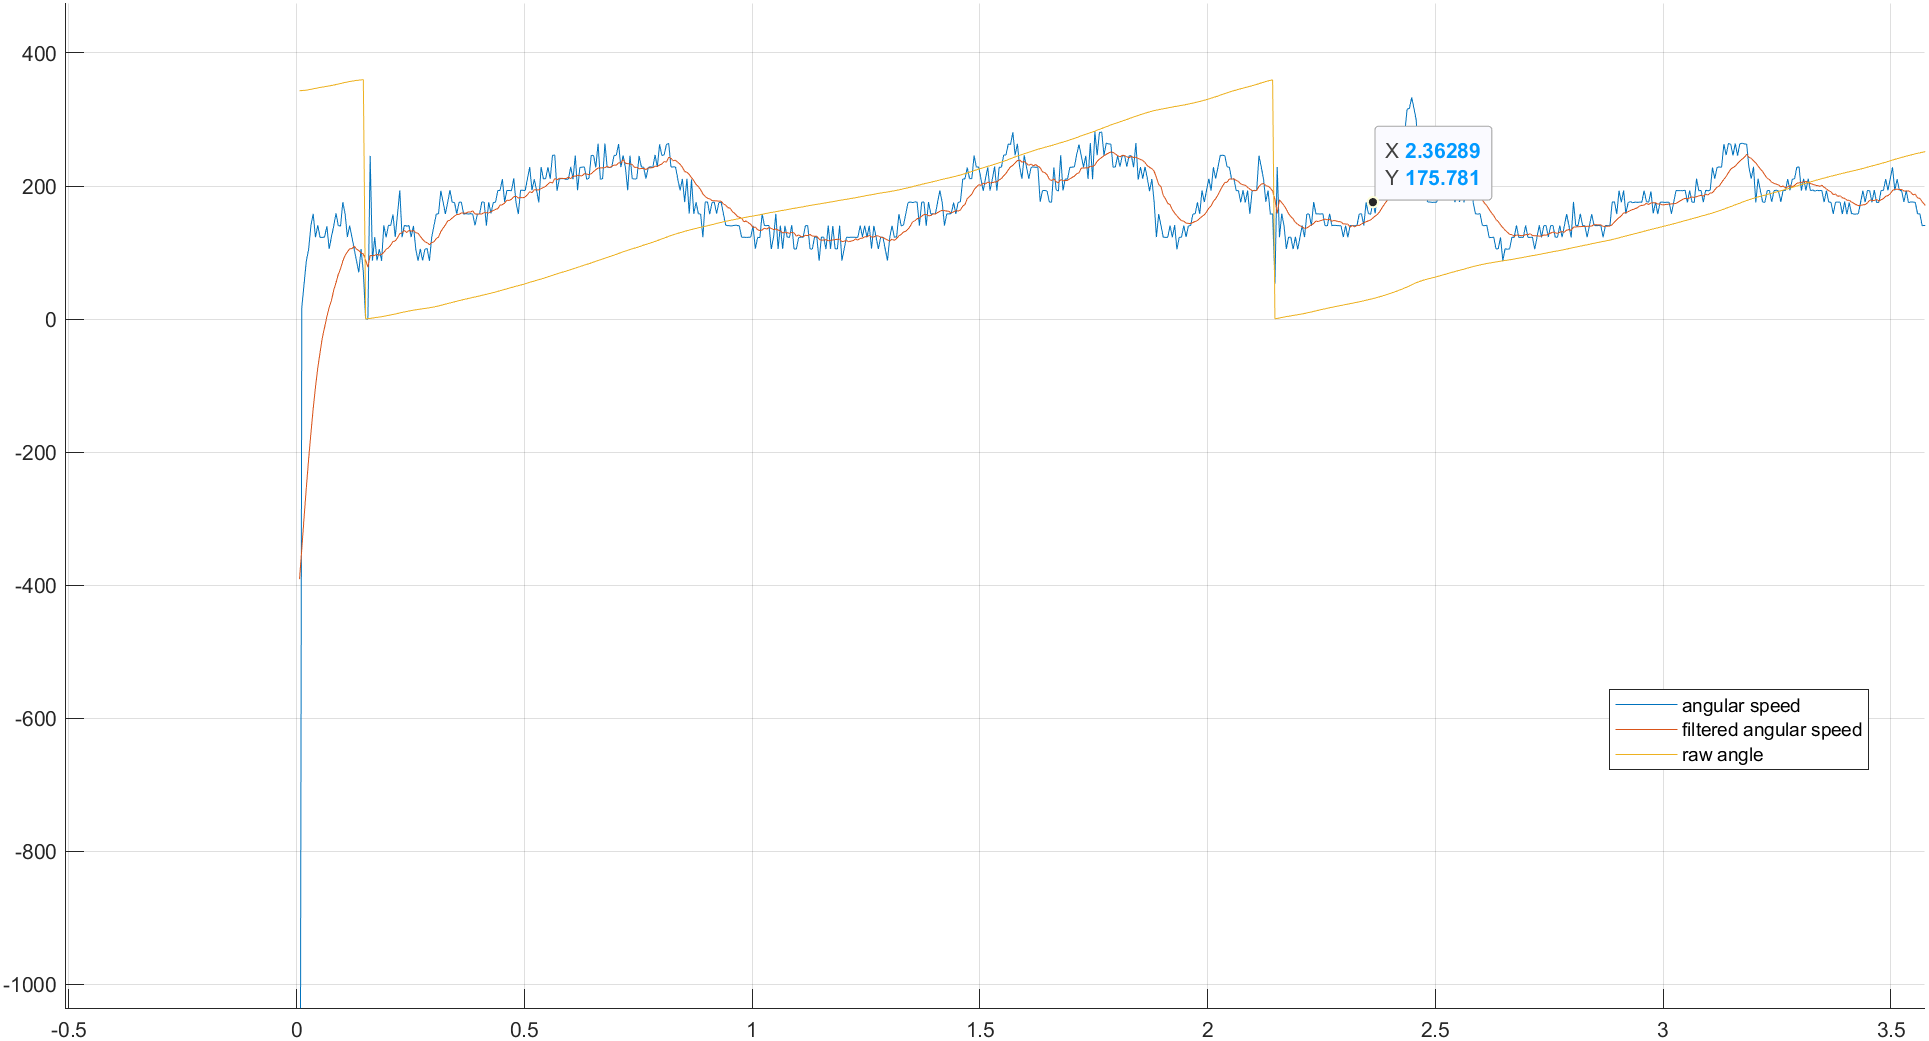
\includegraphics[width=3cm]{figures/inertie_roue.png}
    \caption{Vitesse angulaire (degrés/s) de la roue en fonction du temps (s).}
\end{figure}

Les données constructeurs fournissent une relation 
linéaire entre la vitesse angulaire et le couple d'entrée. $$\omega = a - b\tau$$

On a essayé d'exploiter le théorème du moment cinétique à l'unité roue+rotor:

$$I_w^y\dot{\omega} = \tau = \frac{a}{b} - \frac{\omega}{b}$$
$$\dot{\omega} +  \frac{\omega}{T} = \frac{a}{T} \text{  où  } T=I_w^yb$$


\paragraph{Estimation des constantes électriques}
La résistance et l'inductance interne du moteur ont été trouvées sur Internet 
\href{https://forum.pololu.com/t/mechanics-and-electrical-parameters/18153/2}{ici}.

\chapter{Implémentation du contrôleur en Arduino}

% \printbibliography

\end{document}
